\subsection{Experimento 2}

%Habria que poner la foto del experimento reaaaaal


Para el segundo experimento de este práctico, se plantea realizar una medición indirecta de la resistencia de una probeta (cable). Para esto se establecerá una corriente fija a través de esta y luego se medirá la tensión a los bornes de la probeta para así emplear la Ley de Ohm y obtener el valor de la resistencia.

En la figura \ref{fig:CircExp2}, se puede apreciar el circuito teórico propuesto para este experimento. 

\begin{figure}[H]
    \centering
    \begin{circuitikz} [scale=1,american, transform shape]
\def\scal{1};
\draw (0,-2) to[I] (0,2)  (4.5,2) edge[dashed] (7.5,2) (0,2) to[short,-o] (4.5,2) ;
\draw (7.5,2) to[short,o-] (8,2)to[R, l=$R_{probe}$] (8,-2) (7.5,-2) edge[dashed](4.5,-2) (4,-2) to[short,-o](4.5,-2) (8,-2) to[short,-o](7.5,-2);
\draw (4,2) to[rmeterwa, t=V, v=$v$, o-o] (4,-2);
\draw (4,-2) to[rmeterwa, t=I, i=$i$, o-] (0,-2);

\end{circuitikz}{}
    \caption{Circuito experimento 2}
    \label{fig:CircExp2}
\end{figure}

Además de esta medición, se realizarán los cálculos necesarios para determinar la incertidumbre en esa medición.

En este ensayo, se emplearon algunos instrumentos provistos por el laboratorio, entre ellos: una fuente de corriente con una tensión de alimentación de 12 V y la probeta, que consistía en un tramo de cable enrollado de 20 m $\pm$ 20cm de largo, con un arrollamiento no inductivo (para disminuir al máximo los posibles efectos auto inductivos del cable). Además de esto, se utilizaron dos multímetros de la marca UNI-T. El primer multimetro utilizado era un modelo UT890C, utilizado como miliamperímetro y el segundo fue un modelo UT33C, empleado como voltímetro. 

Antes de realizar el experimento se decidió medir la resistencia de la probeta de manera directa, con el multímetro configurado para comprobar continuidad. Este indicaba que efectivamente había continuidad y que el cable tenía una resistencia de $1.5 \Omega$. 

\subsubsection{Mediciones}

Se conecto la fuente de alimentación, de 12 V, al circuito de la fuente de corriente. Luego se conectaron los bornes de salida de esta, uno a la probeta y el otro al multímetro que mediría la corriente que circula por la probeta. Por supuesto, el otro extremo de la probeta y la otra punta del multímetro fueron conectadas entre sí (figura \ref{fig:foto2}).

\begin{figure}[h!]
    \centering    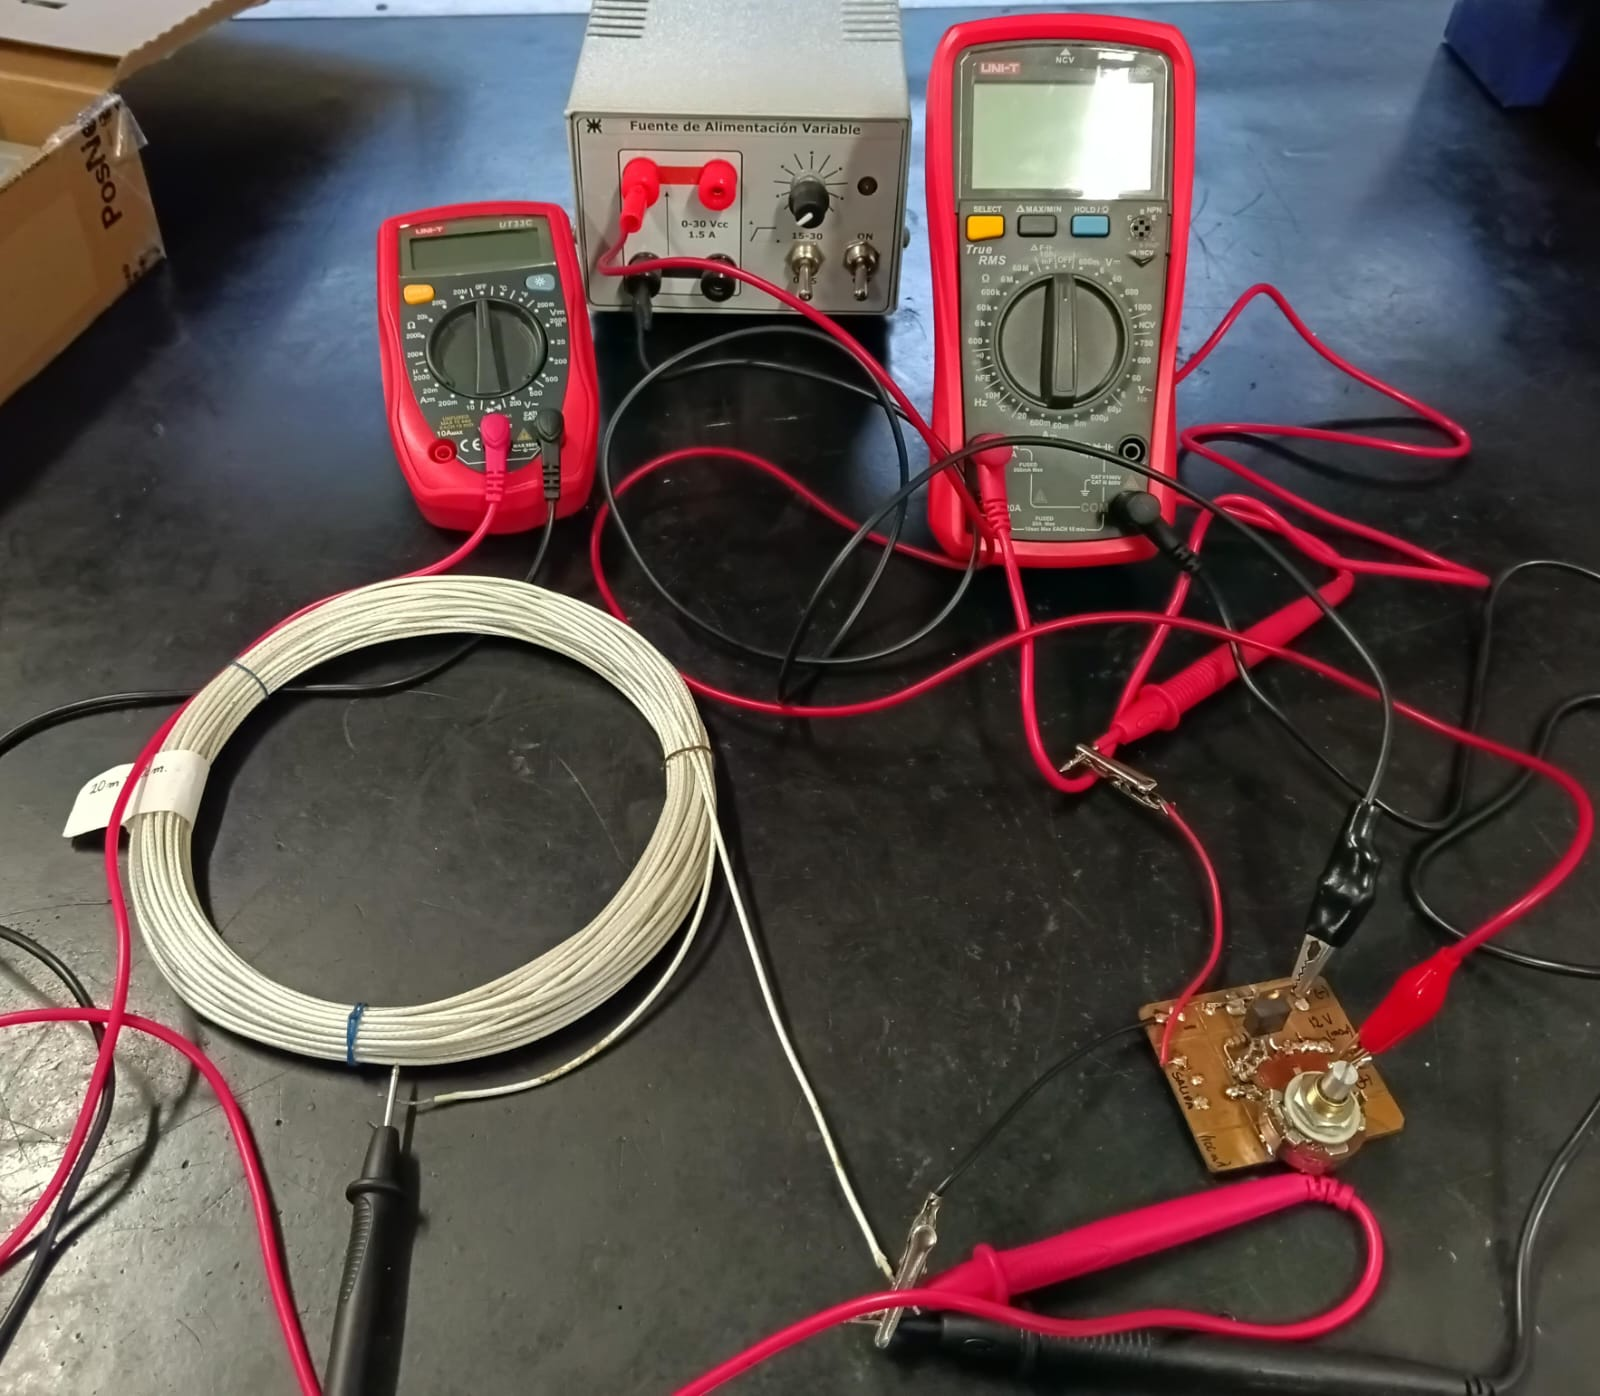
\includegraphics[width=0.5\textwidth]{Imagenes/WhatsApp Image 2024-04-11 at 18.13.00.jpeg}
    \caption{Circuito experimento 2}
    \label{fig:foto2}
\end{figure}

Se estableció una corriente de 100 mA a través de la probeta y se procedió a medir la diferencia de potencial que había entre sus bornes. A partir de este valor se calculó la resistencia del cable cómo se ve a continuación en la tabla \ref{tab:exp2a}.


\begin{table}[h!]
    \centering
    \begin{tabular}{|c|c|}
    \hline
        V & 101 $mV$ \\
    \hline
        I & 100 $mA$ \\
    \hline
        R = V/I & 1.01 $\Omega$ \\ 
    \hline
        \end{tabular}
        \def\tablename{Tabla} 
        \caption{Mediciones sobre la probeta}
        \label{tab:exp2a}
\end{table}

Se obtuvo como resultado un valor de 1.01 $\Omega$, sin embrago, aún queda analizar el nivel de incertidumbre que contiene esta medición. 

\subsubsection{Cálculo de Incertidumbre}

Al realizar una medición indirecta se debe tener en cuenta que la incertidumbre del valor calculado, se verá afectada por los errores de las mediciones implicadas. Por lo tanto, para el cálculo de la incertidumbre en la medición de la resistencia, habrá que tener en cuenta la incertidumbre en las mediciones de corriente y tensión.

El valor de la resistencia resulta ser el cociente entre la tensión y la corriente, por ende, el error relativo máximo total es la suma de los errores relativos máximos parciales, es decir:

\begin{equation}
    \frac{\Delta R}{R} = \frac{\Delta V}{V} + \frac{\Delta I}{I}
    \label{sumaErr}
\end{equation}

Los errores máximos relativos se calculan a partir de las mediciones efectuadas, teniendo en cuenta las especificaciones del multímetro utilizado. 

Antes de calcular el error máximo relativo, debemos averiguar el error de cada medición. Para esto se utilizan los datos que cada fabricante indica en el manual del instrumento. 

La medición de corriente fue efectuada con el miliamperímetro del tester UT890C en el rango de 600 mA. Las especificaciones para el cálculo de la incertidumbre ($\Delta I$) de este las podemos encontrar en el Anexo \ref{sec:Información Instrumentos} en la tabla \ref{tab:DCI_UT890C}. En base a esto, el cálculo quedaría así:

\begin{equation}
    \Delta I = \pm \left( \cfrac{1.2 \cdot 100 [mA]}{100} + 0.5 [mA] \right) = \pm 1.7 [mA]  
\end{equation}

En el caso de la tensión, que fue medida con el voltímetro del tester UT33C en el rango de 200 mV y cuyas especificaciones se pueden ver en la tabla \ref{tab:DCV_UT33C} del Anexo \ref{sec:Información Instrumentos}, la incertidumbre resultó ser:

\begin{equation}
    \Delta V = \pm \left( \cfrac{0.5 \cdot 101 [mV]}{100} + 0.2 [mV] \right) = \pm 0.705 [mV]  
\end{equation}

Con los valores recién obtenidos y mediante lo calculado siguiendo la ecuación \ref{sumaErr}, se confeccionó la tabla \ref{tab:exp2b}, presentada a continuación.

\begin{table}[h!]
    \centering
    \scalebox{1}{
    \begin{tabular}{|c||c|c|c|c|}
    \hline
         ---- & $x$ & $\Delta x$ & $\cfrac{\Delta x}{x}$ & $\cfrac{\Delta x}{x} \cdot 100$ \\
    \hline
        V & 101 $mV$ & 0.705 $mV$ & $6.98 \cdot 10^{-3}$ & $0.698 \%$ \\
    \hline 
        I & 100 $mA$ & 1.7 $mA$ & 0.017 & $1.7 \%$ \\
    \hline
        R = V/I & 1.01 $\Omega$ & $24.2 \cdot 10^{-3}$ $\Omega$ & $23.98 \cdot 10^{-3}$ & 2.398\% \\
         
    \hline
        \end{tabular}}
        \def\tablename{Tabla} 
        \caption{Incertidumbre y error relativo de las mediciones sobre la probeta}
        \label{tab:exp2b}
\end{table}

La incertidumbre de la resistencia ($\Delta R$) fue obtenida luego de emplear la ecuación \ref{sumaErr} y multiplicar el resultado por el valor de resistencia calculada. 

\begin{equation*}
    \frac{\Delta R}{R} = \frac{\Delta V}{V} + \frac{\Delta I}{I}
    \hspace{0.5cm}
    \Longrightarrow
    \hspace{0.5cm}
    \frac{\Delta R}{R} = 6.98 \cdot 10^{-3} + 0.017 = 23.98 \cdot 10^{-3}
\end{equation*}

\begin{equation*}
    \Delta R = 23.98 \cdot 10^{-3} \cdot 1.01 [\Omega] = 24.2 \cdot 10^{-3} [\Omega]
\end{equation*}

Entonces, como resultado final teniendo en cuenta la incertidumbre queda:

\begin{equation*}
    R_{probe} = 1.01 \pm 0.0242 [\Omega]
\end{equation*}

En base a estos resultados, se puede decir que la medición de la resistencia por este método tiene una precisión bastante buena, teniendo un error de solamente unos cuantos miliohm, a diferencia de la escala más baja del multímetro con el que la medimos al principio, que tiene una incertidumbre de al menos 0.5 $\Omega$ (fijos), más el error porcentual del 0.8$\%$ sobre la medición (ver tabla \ref{tab:DCR_UT33C}, del Anexo \ref{sec:Información Instrumentos}).